%! Author = Miszka and Tamarka
%! Date = 10.03.2022

% Preamble
\documentclass[11pt]{amsart}

% Packages
\usepackage{float}
\usepackage[T1]{fontenc}
\usepackage{geometry}
\usepackage{parskip}
\usepackage{amsmath}
\usepackage{amsfonts}
\usepackage{amsthm}
\usepackage{amssymb}
\usepackage{titling}
%\usepackage{itemize}
\usepackage{enumerate}
\usepackage{multirow}
\usepackage{graphics}
\usepackage{graphicx}
\usepackage{caption}
\usepackage{array}
\usepackage{xcolor}
\usepackage{subcaption}


\graphicspath{ {./fig/} }


%\setlength{\droptitle}{-2cm}
%\newgeometry{tmargin=1.9cm, bmargin=1.9cm, lmargin=1.7cm, rmargin=1.7cm}

\DeclareMathOperator*{\argmin}{arg\,min}

\newcommand{\tami}[1]{{\textcolor{magenta}{#1}}}
\newcommand{\domi}[1]{{\textcolor{green}{#1}}}

\author{Tamara Frączek, Dominik Mika}
\title{Methods of classification and dimensionality reduction - Report 1}
\date{\today}

% Document
\begin{document}
\maketitle


\section{Introduction}

\subsection*{Statement of the problem}

In this task we have to create a movie recommender system for our users.
\domi{We have users who rated some movies}.
Of course, not every user rated every movie and it is our task to fill those gaps.
So if one user hasn't seen one movie, we want to predict how he would like it.



%some movies and some information about how our users rate our movies.
%Since, of course, not every user rated every movie, we want to predict how they would like the movies from our list.

%We have the data containing information how users rate some movies.
%Our task is to create a recommender system, so having only some data we want to predict all ratings.

For this purpose we build few algorithms using different methods of predicting.
%These methods are described in ...
Of course different methods will give us different results (errors).
Our task is to tune parameters of those methods and try to get the best possible ratings prediction.



\subsection*{Description of methods}

In this problem, we use different methods which are subset of PCA methods. They are often used for dimensionality reduction and matrix factorization.

\subsubsection*{SVD1}

This method gets a $n \times d$ dimensional matrix $Z$ and approximate it by a different matrix $\tilde{Z}$.
Since we want somehow $\tilde{Z}$ to maintain only ''the most important'' information from $Z$, then the rank of $\tilde{Z}$ is to be much smaller than rank of $Z$.
Precisely, we want to find matrix $\tilde{Z}_r$ of rank $r$ ($r < rank(Z)$ and $r$ is a parameter), so that $\|Z - \tilde{Z}_r\|$ is small.

Using SVD decomposition $Z = U \Lambda^{\frac{1}{2}} V^T$ we construct $\tilde{Z}$ as
\[\tilde{Z}_r = U_r \Lambda_r^{\frac{1}{2}}V_r^T,\]
where $\Lambda_r$ contains $r$ biggest eigenvalues of $Z$ and $U_r$, $V_r$ contains only columns corresponding to those eigenvalues.

\subsubsection*{SVD2}

It is an iterative method.
We perform SVD1 on matrix $Z$, then on the result of first SVD1 and so on.
The algorithm can be stopped after a fixed number of iterations or some stop condition can be established.


\subsubsection*{NMF}

Similarly as in SVD1 the method obtain a $n \times d$ dimensional matrix $Z$ and approximate it by $\tilde{Z}$.
This time $\tilde{Z}$ is constructed as $\tilde{Z}_r = W_r H_r $, where $W_r$ and $H_r$ are matrices with non-negative elements ($W_r$ has $r$ columns and $H_r$ has $r$ rows).
Precisely, we look for such $W_r$ and $H_r$ that $\|Z - W_r H_r \|^2$ is the smallest, where $\|A\|^2 = \sum_{i, j} A_{ij}^2$.

\subsubsection*{SGD}

This method, similarly as previous ones want to estimate matrix $Z$ with a product of matrices
$W$ and $H$, but not necessarily obtaining the whole matrix $Z$.

Let's assume that we have only some values of $z_{ij}$ and let call those pairs $(i,j)$ where we know the value of $Z$ as $I$.
We look for
$$\argmin_{W, H} \sum_{(i,j)\in I} (z_{ij} - w_i^T h_j)^2 + \lambda(\|w_i^T\|^2 + \|h_j\|^2),$$
where $h_j$ is $j$-th column of $h$, $w_i^T$ is $i$-th row of $W$ and $\lambda > 0$ is a parameter.
So roughly speaking we look for $W$ and $H$ such that $Z \approx WH$ for elements known in $Z$, but also we want $W$ and $H$ to have quite small values (it gives us the part of sum with parameter $\lambda$).

\tami{opis metody...}

\section{Implementation}

\subsection*{Description of the data}

Our data contains information 100837 ratings - exactly 610 users rated 9724 movies.
The columns are: \textsf{userId} (integer), \textsf{movieId} (integer) and \textsf{rating} (integer), where \textsf{userId} is a unique user id and \textsf{movieId} is a unique movie id.


We keep this data in two-dimensional matrix of size $n \times d$ where $n$ is the number of users and $d$ is the number of movies.
In element $(i,j)$ we put the rate of the user $i$ of the movie $j$.
If the user $i$ haven't rated the movie $j$ we leave the element empty.


\subsection*{Performing methods}

\tami{??tutaj jakaś intuicja po co dzielić dane??}

So to be able to evaluate the quality of the programs we split our data to two parts: train set and test set.
The train set is used to build the programs.
And the test set is used to evaluate how our programs work.


To give our programs enough information about every user we split the data so that the train set contain 90\% of ratings of each user (and the test set the remaining ones).
\tami{tutaj coś o tym, że będziemy to powtarzać??}

Let call the matrix containing the data from the train set as $\boldsymbol{Z}$ and the matrix containing the data from the test set as $\boldsymbol{T}$.


\subsection*{Quality of the system}

Assume that our algorithm return a matrix $\boldsymbol{Z}^{'}$.
Then the quality of our programs is computed as \textbf{root-mean square error}
\[\textsf{RMSE} =
\sqrt{\frac{1}{|\mathcal{T}|} \sum_{(u,m) \in \mathcal{T}} \left(\boldsymbol{Z}^{'}[u,m] - \boldsymbol{T}[u,m] \right)^2}\]
where $\mathcal{T}$ contains pairs $(u,m)$ from test set.


\subsection*{Imputing the missing data}

Since three of our methods (SVD1, SVD2 and NMF) are given a full matrix $\boldsymbol{Z}$ then they need the missing data to be imputed before performing.

We decided to impute the data in 4 different ways:
\begin{itemize}
    \item putting 0 everywhere,
    \item putting global mean everywhere,
    \item putting row mean,
    \item putting weighted row and column mean ($\alpha \cdot \text{\textsf{col\_mean}} + (1-\alpha) \cdot \text{\textsf{row\_mean}}$, where $\alpha$ is a parameter).
\end{itemize}

\tami{tutaj przemyślenia na temat tego czemu niektóre metody działają lepiej i dlaczego}

\section{Parameters tuning and results}

\tami{coś o tym, że metody pozostawiaja trochę dowolności?}

Before performing our methods and obtaining results we have to set some parameters.

First of all, all the methods need a parameter $r$, which is the rank of matrices in $Z$ decomposition.
SGD needs also learning rate and $\lambda$.
And iteration methods need maximum of possible iterations or a stop condition.

What's more, for all of our methods we want to choose optimal $\alpha$ in the last method of imputing data.



\subsection*{SVD1}

\tami{co tu napisać}

\tami{napisać co to jest to weighted}

At the beginning we consider only \tami{...}

Below, we present a graph showing dependence of RMSE on $r$.

\begin{figure}[H]
\centering
\begin{minipage}{.5\textwidth}
  \centering
  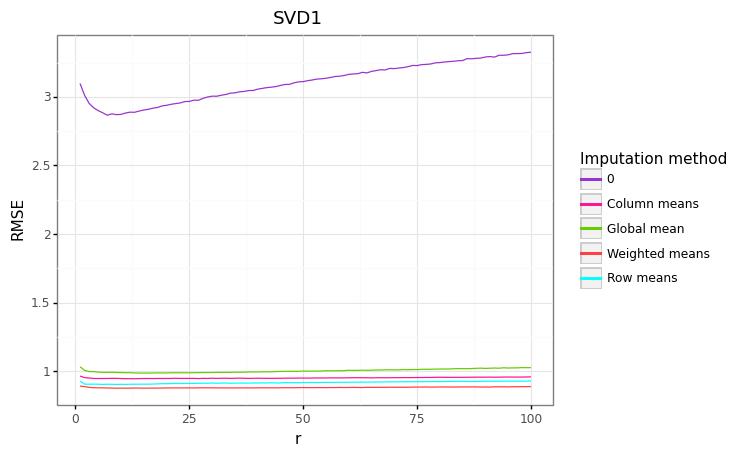
\includegraphics[scale=0.43]{svd1_1}
%  \captionof{figure}{A figure}
%  \label{fig:test1}
\end{minipage}%
\begin{minipage}{.5\textwidth}
  \centering
  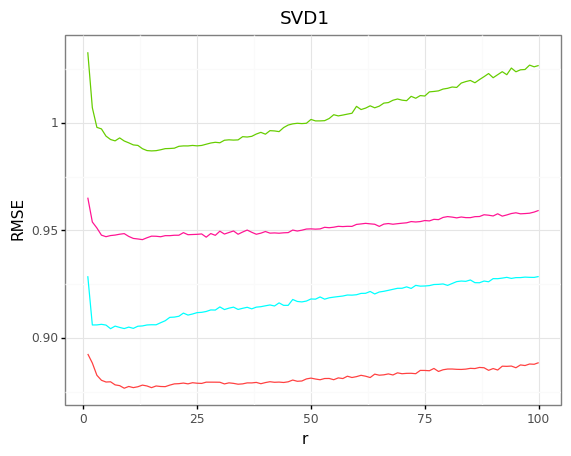
\includegraphics[scale=0.43]{svd1_2}
%  \captionof{figure}{Another figure}
%  \label{fig:test2}
\end{minipage}
\end{figure}

Also we present a table with the lowest RMSE for every imputation method and the parameter $r$ that gave it.
\begin{table}[H]
\begin{tabular}{c|ccccc}
& 0 & column means & global mean & weighted means & row means \\
\hline
$r$ & 7 & 13 & 15 & 9 & 6 \\
RMSE & 2.866 & 0.946 & 0.987 & 0.877 & 0.904 \\
\end{tabular}
\end{table}
%wnioski, że ma wpływ jak uzupełniamy
%jakieś wnioski, te zera beznadziejne
%że weighted wypadają najlepiej i chcemy to alfa dobrać optymalnie

First of all, we observe that as we expected the imputation method does matter.
It is most clearly seen looking at RMSE of data filled with zeros, that for the best $r$ is around $2.9$.
Other methods also differ a lot.
The lowest RMSE obtain the data filled with weighted data.
That's why we may suspect that optimizing $\alpha$ can give even better results.

%wprowadzenie, że dobieramy alfa
%no i ten rysunek wyżej nam pozwala obciąć r
%że robimy minimalizację po dwóch parametrach

To get optimal result we perform optimization with respect to two parameters: $\alpha$ and $r$.
As we can see on the picture above only $r$ between $0$ and $50$ give some reasonable results, so we consider only those (we could use all $r$, but it is time consuming).
Below, we present graph showing dependence of RMSE on $\alpha$ and $r$ for data \tami{...}

\begin{figure}[H]
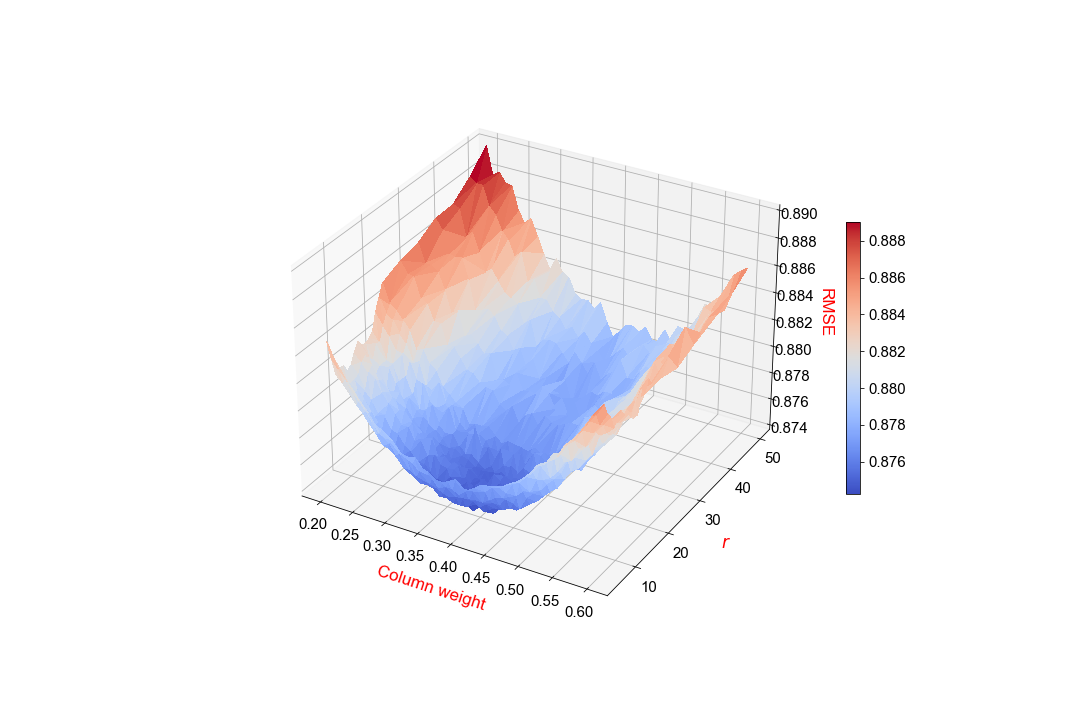
\includegraphics[scale=0.45]{fig/svd1_r_w}
\label{fig:figure}
\end{figure}

Below we present also table with \tami{...} lowest RMSE and pairs $(\alpha, r)$ that gave those.
\begin{table}[H]
\begin{tabular}{cc|c}
\toprule
 $\alpha$ &  $r$ &     RMSE \\
\midrule
\hline
       0.39 & 10 & 0.873987 \\
       0.38 & 10 & 0.874244 \\
       0.42 & 10 & 0.874274 \\
       0.36 & 10 & 0.874449 \\
       0.39 & 11 & 0.874469 \\
\bottomrule
\end{tabular}
\end{table}

As we can see 10 seems to be the best $r$ and 0.39 seems to be the best $\alpha$.
Also in all those results $(\alpha, r)$ are close to them.
\tami{So $\alpha = 0.39$ and $r = 10$ are parameters that we use to perform this method further in the report.}

Since in columns we keep indexes of movies, it means that our filled data take a bit more information from user ratings mean than from the movie ratings mean.
That is probably logical \tami{...}

To conclude this subsection we present our best results obtained using these methods.
\tami{which means what}

\tami{tabelka z najlepszymi wynikami}


\subsection*{SVD2}
In this case we want to proceed as in SVD1 case.

\tami{??In SVD2 we make a correction -- czy to tu}

stop condition



\begin{figure}[H]
\centering
\begin{minipage}{.5\textwidth}
  \centering
  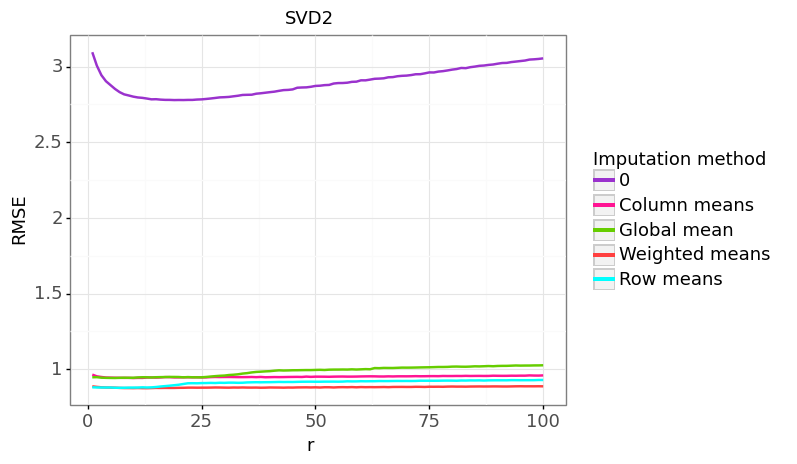
\includegraphics[scale=0.43]{svd2_1}
%  \captionof{figure}{A figure}
%  \label{fig:test1}
\end{minipage}%
\begin{minipage}{.5\textwidth}
  \centering
  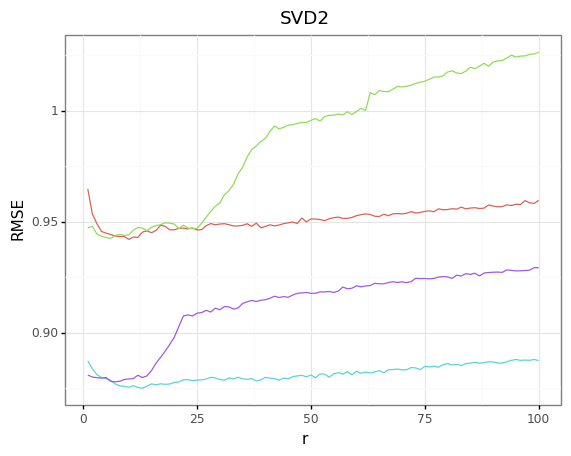
\includegraphics[scale=0.43]{svd2_2}
%  \captionof{figure}{Another figure}
%  \label{fig:test2}
\end{minipage}
\end{figure}

\begin{table}[H]
\begin{tabular}{c|ccccc}
& 0 & column means & global mean & weighted means & row means \\
\hline
$r$ & 19 & 10 & 6 & 13 & 7 \\
RMSE & 2.779 & 0.942 & 0.942 & 0.875 & 0.878 \\
\end{tabular}
\end{table}

\begin{figure}[H]
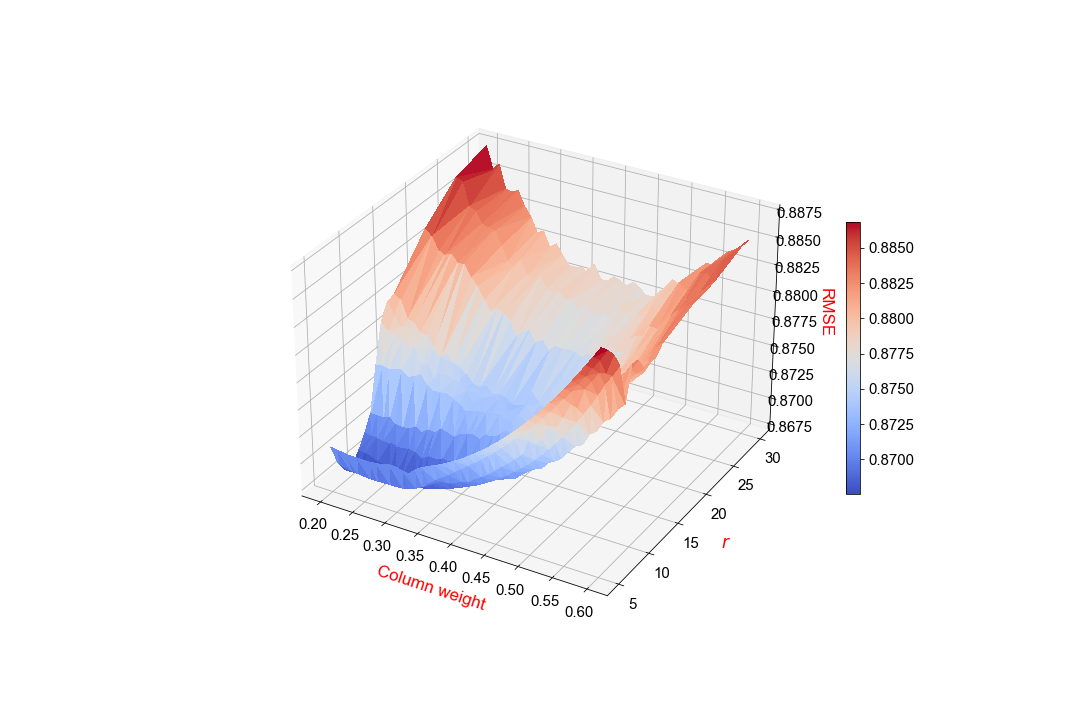
\includegraphics[scale = 0.45]{svd2_r_w}
\end{figure}

\begin{table}[H]
\begin{tabular}{rrr}
\toprule
$\alpha$ &  $r$ &     RMSE \\
\midrule
\hline
       0.25 &  8 & 0.867393 \\
       0.26 &  8 & 0.867397 \\
       0.24 &  8 & 0.867402 \\
       0.27 &  8 & 0.867410 \\
       0.28 &  8 & 0.867494 \\
\bottomrule
\end{tabular}
\end{table}

\subsection*{NMF}

In this case since we have only $r$ and $\alpha$ to find, we proceed in exactly the same way as in the case of SVD.
So, firstly we present a graph showing dependence of RMSE on $r$. \tami{in some cases...}

\begin{figure}[H]
\centering
\begin{minipage}{.5\textwidth}
  \centering
  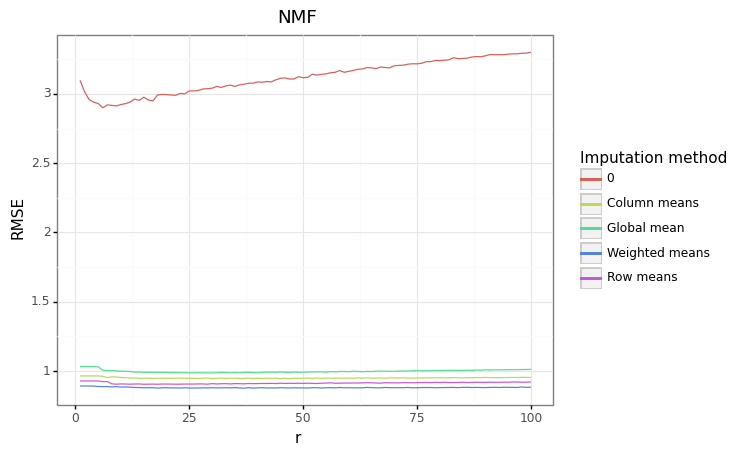
\includegraphics[scale=0.43]{nmf_1}
%  \captionof{figure}{A figure}
%  \label{fig:test1}
\end{minipage}%
\begin{minipage}{.5\textwidth}
  \centering
  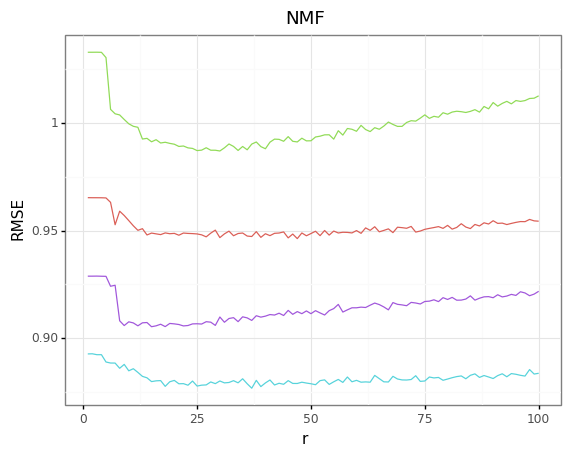
\includegraphics[scale=0.43]{nmf_2}
%  \captionof{figure}{Another figure}
%  \label{fig:test2}
\end{minipage}
\end{figure}

Comparing this graph to the graph for SVD we can see that \tami{tutaj o tym, że jest bardziej takie postrzępione}

Below we also present a table with the lowest RMSE for every imputation method and the parameter $r$ that gave it.

\begin{table}[H]
\begin{tabular}{c|ccccc}
& 0 & column means & global mean & weighted means & row means \\
\hline
$r$ & 6 & 47 & 30 & 37 & 15\\
RMSE & 2.900 & 0.946 & 0.987 & 0.877 & 0.905 \\
\end{tabular}
\end{table}

\begin{table}[H]
\begin{tabular}{cc|c}
\toprule
$\alpha$ &  $r$ &     RMSE \\
\midrule
\hline
       0.40 & 37 & 0.874794 \\
       0.41 & 37 & 0.874817 \\
       0.39 & 18 & 0.874841 \\
       0.39 & 37 & 0.874848 \\
       0.40 & 18 & 0.874849 \\
\bottomrule
\end{tabular}
\end{table}

As we can see the parameters $r$ are in general bigger than in previous cases.
\tami{czy będą bardziej porostrzelane}

Now we pefrorm the optimization with respect to $\alpha$ and $r$ and present a graph showing the results.

\begin{figure}[H]
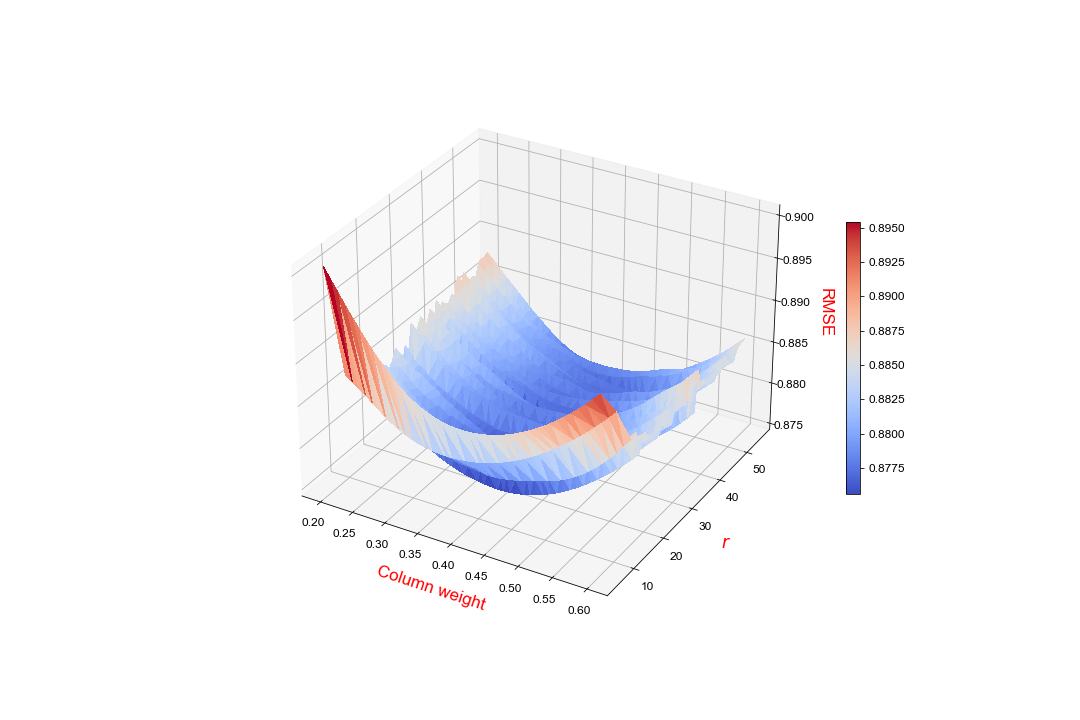
\includegraphics[scale = 0.45]{nmf_r_w}
\end{figure}

\tami{tabelka z najlepszymi r i alpha}
\tami{jakie r i alpha wybieramy}

\tami{tabelka z najlepszymi wynikami}

\subsection*{SGD}

\begin{figure}[H]
\centering
\begin{minipage}{.5\textwidth}
  \centering
  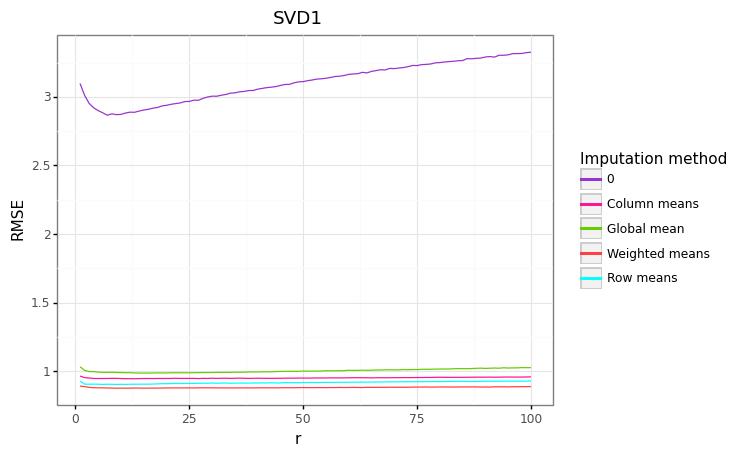
\includegraphics[scale=0.43]{svd1_1}
%  \captionof{figure}{A figure}
%  \label{fig:test1}
\end{minipage}%
\begin{minipage}{.5\textwidth}
  \centering
  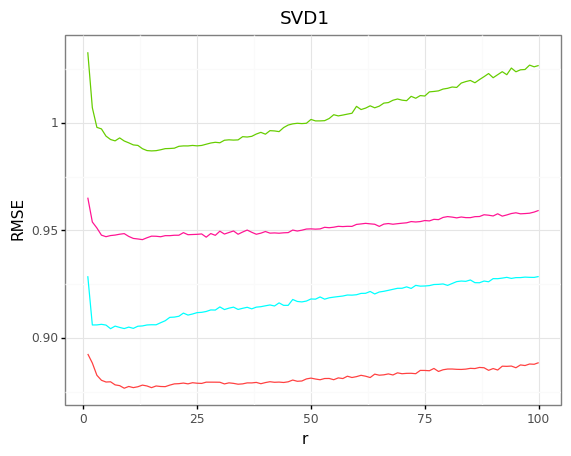
\includegraphics[scale=0.43]{svd1_2}
%  \captionof{figure}{Another figure}
%  \label{fig:test2}
\end{minipage}
\end{figure}



\section{}

\section{Conclusions}



\end{document}